\documentclass[a4paper,titlepage]{article}

\usepackage{amsmath, amssymb}

\usepackage[T1,T2A]{fontenc}
\usepackage[utf8]{inputenc}
\usepackage[UKenglish]{babel}

\usepackage{graphicx}
\usepackage[justification=centering]{caption}
\usepackage[hidelinks]{hyperref}
\usepackage[nottoc,numbib]{tocbibind}
\usepackage{algorithm}
\usepackage{algpseudocode}
\usepackage{booktabs}

\hyphenation{Du-rak Krau-dia Ap-prox-i-ma-tors Non-lin-ear Tu-ple Tu-ples Pa-ram-e-ter-ized Stochas-tic Op-ti-miza-tion Sub-game}

\widowpenalty=300
\clubpenalty=300

\DeclareMathOperator{\Expectation}{\mathbb{E}}
\DeclareMathOperator*{\argmax}{arg\,max}
\DeclareMathOperator*{\argmin}{arg\,min}

\newcommand{\Exp}[3]{\Expectation_{#1} \left[ #2 \ \middle| \ #3 \right]}
\newcommand{\Ex}[2]{\Expectation_{#1} \left[ #2 \right]}

\newcommand{\expn}[2]{{#1}\mathrm{e}{#2}}

\title{Reinforcement Learning for Durak \\ \medskip \large{Bachelor's Thesis on Reinforcement Learning}}
\author{Jan Ebert \smallskip \\ \\ \small{Cognitive Informatics} \\ \small{Faculty of Technology}}
\date{\today}

\pagenumbering{roman}

\begin{document}

\maketitle

\setcounter{page}{2}
\thispagestyle{empty}
\noindent
\textbf{Declaration of Authorship} \medskip

\noindent
This thesis and the corresponding code have been written solely by myself, Jan~Ebert. All sources used have been cited and referenced. \bigskip

\noindent
\makebox[3cm]{\hrulefill} \hspace{0.2cm} \makebox[4cm]{\hrulefill}

\noindent
\makebox[3cm][l]{\textit{Signature}} \hspace{0.2cm} \makebox[4cm][l]{\textit{Place and date}}

\begin{abstract}
\setcounter{page}{3}
I adapt the successful deep deterministic policy gradient algorithm to the card game durak. The proposed model is supposed to work for most variants of durak. With only miminal prior knowledge, the model successfully learns durak's rules and demonstrates better results than simply playing at~random.
\end{abstract}

\setcounter{page}{4}
\thispagestyle{empty}
\tableofcontents

\newpage

\pagenumbering{arabic}

\section{Introduction}

Reinforcement learning~-- and machine learning in general~-- is one of the most progressive scientific fields in present time. Learning like a human by trial and error is fascinatingly useful and can have large influences in a lot of very different subjects. Because computers are much faster at calculating than a human and can concentrate solely on the problem at hand, not needing time to, for example, do the dishes, they can find correlations that even experts of certain topics have not discovered yet; simply by magnitude of observations. Underlining why machine learning is so important, Andrew Ng, who founded the Google Brain project, gives this introduction for an online course on machine learning: ``Machine learning is the science of getting computers to act without being explicitly programmed. In the past decade, machine learning has given us self-driving cars, practical speech recognition, effective web search, and a vastly improved understanding of the human genome. Machine learning is so pervasive today that you probably use it dozens of times a day without knowing it. Many researchers also think it is the best way to make progress towards human-level AI.''~\cite{mlquote}
In contrast to supervised and unsupervised machine learning methods, the greatest benefit of reinforcement learning is that data is created by the system itself. Huge amounts of data are not needed prior to creating a reinforcement learning system. The system simply finds its own, relevant data~-- sometimes even while~learning.

However, reinforcement learning is also very complex: Even after having chosen the right reinforcement learning method for the current domain, many very different parameters have to be tuned to get acceptable results. To try and understand reinforcement learning and how to avoid its pitfalls, I model the Russian card game durak and let an agent learn it. It does that by first playing against players that only execute random actions and then, when it has learned enough to understand the basics of the game, by playing and improving against itself. I want to solve the game without explicitly modeling it by calculations of probabilities. The agent simply plays the game and learns to find regularities and an optimal strategy without further interaction from my~side.

Durak is an interesting game for this task for many reasons: First of all, it has many variables. In durak, the amount of cards in the deck, amount of cards in hand or even amount of players can vary. The amount of players in the game varies even while playing: Winners are removed from the game while the others continue to compete. It is a competitive multi-agent game with limited information up until the end when the remaining players have perfect information. In each game state, a selection from a lot of very different actions can be made. Each decision might end up changing the end result of the game.
Because durak is played in real time, it is interesting to see how the agent deals with actions of other players that influence the game's state independently from the agent.
Also, durak might simply be a game of luck. Testing whether skill is involved and how much it can influence the outcome of a game will be tested by the learning~agent. \medskip

The two biggest challenges that have to be addressed in this thesis are the chosen reinforcement learning method and how to handle parameterized actions. Other challenges include the representation of the game's states (information about the game necessary for the agent to make a smart decision), the reward function which shapes the agent's behaviour by evaluating its actions and how to set up the experiments in a way that provides a lot of information while still being time efficient. After all these problems are solved, it is still not given that the reinforcement learning actually works due to its complexity. Even if it does work, the mileage may vary and results could be~unsatisfactory. \medskip

I am now first going to explain the rules and variations of durak. Then I will delve into the theory of reinforcement learning and explain which method I am going to be using. After that, I present how and why I modeled the game's representations the way I did. With this theoretical basis, I then go into detail on the implementation of the program and finally I evaluate different experiments I conducted to find the most optimal behaviour the system could achieve. I finish with a conclusion and explain what new understanding this thesis does and does not~yield.

\newpage

\section{Durak}

Durak, like most older card games, can have a lot of variations, starting with the number of cards and players. A standard 52-card deck is used to play. The classic Russian version is played with 36~cards by removing the cards 2 to~5 of every suit. Durak can be played with any amount of cards divisible by four though (as there are four suits). Multiple decks can even be combined, duplicates are not treated~differently.

The goal of the game is to get rid of one's cards so as not to be the durak (Russian: Дурак, meaning ``fool''). First, a deck is shuffled and each player is dealt six cards (or, for example, only five if there are not enough cards~-- durak is very flexible) and one card is laid on the table for everyone to see. This is the card determining the trump suit for the current game. The deck is placed on the open card as a talon. The revealed card is part of the talon, so the last card drawn is always a trump.
There are two phases in the game: When the talon is not empty, players redraw cards from it and can not yet win. When it has been completely drawn, players can start emptying their hands and ultimately win. However, this is not exactly correct, as in durak, there is no winner, only a loser. I will, however, use the term winner for ``not~loser''. \medskip

The player with the lowest trump begins the game (if there are duplicates and several players have the lowest trump, the next lowest trump could be taken instead). They attack with a card of their choice that the next player in clockwise order then has to defend by placing a card of the same suit with a higher value onto it. The defending player can also use a trump to defend any card except another trump with a higher value. The defender's neighbours, the first and second attacker, can place any card whose value is already on the table as another attack (so the attackers can also instantly place two or more cards of the same value on the table). They can do this until there are either six (or, depending on the hand size, another value) attack cards on the table or as many attack cards as the defender has cards remaining in his hand. In classic durak, only five cards can be placed before the first successful defence but I will do without this~rule.

If the defence is successful, that means that no attacker can or wants to put another card as an attack (they \emph{check}), all cards on the table are removed and the players draw from the talon in order of attackers with the defender always drawing last. The defender then attacks the next player.
If the defending player cannot defend all cards, they must pick up every card on the table and cannot start attacking the next round. Instead, the player coming after the defender begins after the players drew cards like before. When the defender signals that they cannot defend (this is also checking), the attackers can still place (legal) cards that the defender also has to take. As before, the amount of attack cards cannot exceed the hand size or the amount of cards in the defender's hand.
When a player has no cards left, they are out of the game and cannot become durak. In most versions, the finished player's place is taken by the player coming before them only after an attack has ended but in my version, they immediately move up.
Another rule that is not in classic durak is pushing. Pushing means that, when no card has been defended, the defender can put a card of the same value as the attacking card (or cards) next to it (instead of covering it) and \emph{push} the attack to the next player who then has to defend all cards as usual. The new defender's neighbours are the only attackers, so the original first attacker has no further part in the attack (unless they are the defender's neighbour~again).

The last player with cards in hand is the loser and receives the title of ``durak''. They have to shuffle and deal the cards for the next game and are the first to be attacked. When a new player joins the others or someone leaves, it is a new game and the player with the lowest trump begins the game instead as if there was no durak. If no player has a trump in hand, I randomly select a~beginner. \medskip

Durak is also notorious for being a game that allows cheating. Players can place anything they want on the table. Even if they are caught, there is no penalty~-- they just have to take the illegal card(s) back in hand. While this is great for teaching new players the rules of the game, a learning agent would be distracted by it so I will only focus on ``fair''~durak.

In Wikipedia~\cite{wikidurak}, durak refers to the page ``Games of skill'' in its section ``See also''. With the learning agent, I want to test whether that reference is correct. While there is randomness and luck involved in the outcome of a game, the agent should get a higher win rate (non-loss rate) than players acting at~random. \medskip

The version that I will mostly concentrate on in the experiments is a downscaled one played with a deck of 12~cards, 3~cards in hand and only two players.
Pushing and immediate moving up when a player is out is~allowed.

\newpage

\section{Reinforcement Learning}

Reinforcement learning is an area of machine learning trying to model human trial-and-error learning mathematically. Sutton and Barto summarize it like this: ``Reinforcement learning is a computational approach to understanding and automating goal-directed learning and decision-making. It is distinguished from other computational approaches by its emphasis on learning by an agent from direct interaction with its environment, without relying on exemplary supervision or complete models of the environment.''~\cite[p.~15]{book} At time~$t$, an agent interacts with an environment's state~$s_t$ by executing an action~$a_t$ that is chosen based on a learned policy~$\pi$. All states and all actions possible in the environment make up the state space and action space, respectively. A policy can be understood as a mapping from a state to an action that is then taken. After executing the action, the agent receives a reward~$r_t$ and observes a new state~$s_{t+1}$. Learning is based on maximizing the expected, cumulative future reward, also called the \emph{return}. The return is usually discounted by a factor $0 \leq \gamma \leq 1$ to control the agent's foresight. The greater~$\gamma$, the more strongly future rewards are taken into account. Thus, for the return at time~$t$, we~get
\begin{equation*}
  R_t \doteq r_{t+1} + \gamma r_{t+2} + \gamma^2 r_{t+3} + ... = \sum_{k = 0}^{\infty} \gamma^k r_{t+k+1}.
\end{equation*}
These returns can be used to calculate how good taking a certain action~$a_t$ and then following policy~$\pi$ is in a given~state~$s_t$:
\begin{equation*}
  q_\pi(s_t, a_t) \doteq \Exp{\pi}{R_t}{s_t, a_t} = \Exp{\pi}{\sum_{k = 0}^{\infty} \gamma^k r_{t+k+1}}{s_t, a_t},
\end{equation*}
which is the \emph{action-value function} of policy~$\pi$.
$q_\pi$ can be estimated from experience which is key to reinforcement learning.
Also, $q_\pi$ satisfies a recursive relationship called the \emph{Bellman~equation}:
\begin{align*}
  q_\pi(s_t, a_t) &= \Exp{\pi}{R_t}{s_t, a_t} \\
  &= \Exp{\pi}{r_{t+1} + \gamma R_{t + 1}}{s_t, a_t} \\
  &= \Ex{r_{t+1}, s_{t+1}}{r_{t+1} + \gamma \Exp{\pi, a_{t+1} \sim \pi}{R_{t+1}}{s_{t+1}, a_{t+1}}} \\
  &= \Ex{r_{t+1}, s_{t+1}}{r_{t+1} + \gamma q_\pi(s_{t+1}, a_{t+1})},
\end{align*}
where $a_{t+1} \sim \pi$ is the action taken with respect to~$\pi$.
$q_\pi$ can only be written without the second expectation if $\pi$ is deterministic, meaning that $\pi$ does not model probabilities of choosing an action but instead maps to an explicit~action.

We seek an optimal policy~$\pi_*$ that fulfils $q_{\pi_*}(s, a) \doteq \max_\pi q_\pi(s, a)$. If $\pi_*$ is found, the reinforcement learning problem is solved. This optimal policy can only be defined for \emph{finite Markov decision processes}. A reinforcement learning problem is called a Markov decision process if a state can summarize all information that matters for the present and future of the problem. It is a finite Markov decision process if its action and state spaces are finite. However, this is mostly important for the theory of reinforcement learning (which is based on this property) and since durak cannot be viewed as a finite Markov decision process because of its imperfect information and no prior knowledge of the other players' behaviour (which will influence future game states), it is usually okay to not have perfect information as the theoretical ideas and methods can be applied more generally even though they are technically wrong. This means that we do not need a perfect representation of the game's state to achieve good results. We can compare it to humans playing a card game: It is often enough to track only the most important cards instead of every single one. There is no need to remember how many beads of sweat were on a player's forehead when they made a questionable~decision. \medskip

The environment providing each state can be modelled, meaning that for a given state, every probability and expected reward for each new state is defined. These values are used to plan actions by considering all possible future states, their chances of occurring and their reward. This is in contrast to simply learning by trial and error on a simulated model. It is much easier to simulate a complex problem than it is to perfectly model its environment. That is why I am going to concentrate on \emph{model-free} algorithms that rely on simulations instead of doing the Sisyphean work of calculating every single probability of durak. Even though, model-based approaches are more theoretically sound and can be built upon by dynamic programming. Also, model-based approaches can be combined with model-free ones so that the agent might learn the model itself as well.

A central idea of reinforcement learning is that of temporal-difference learning. Changes in training are based on the comparison, or the \emph{difference}, of an old action-value and a new one with an associated reward. The method of only calculating the difference of the old action-value to the directly following action-value (with the associated reward) is called TD(0). TD(1) calculates the difference from the very last action-value received to the first one. In between those two are TD($\lambda$)~methods with $0 \leq \lambda \leq 1$ which weigh future action-values depending on~$\lambda$, similar to the discount factor~$\gamma$. We will focus only on TD(0) which is the basis of the backups considered in this thesis. Backups are changes during learning where new values are calculated from older values. The new value is \emph{backed up} from the old value.
As an example, the  \emph{very} simplified temporal difference loss that the agent will train on is this: $L = (r_t + \gamma q(s_{t+1}, a_{t+1} \sim \pi) - q(s_t, a_t))^2$ (see~\hyperref[sec:ddpg]{section~\ref*{sec:ddpg}})

The balance of exploitation against exploration is a big problem in reinforcement learning. Exploitation is simply taking the action with the most return associated to it, so the acquired knowledge is exploited. But it is also important to consider other actions and learn that they might offer an even better return than the action suggested by the current policy. That is exploration: Trying out new actions and observing whether they are useful. To solve this problem, often, an $\epsilon$-greedy strategy (with $0 \leq \epsilon \leq 1$) is applied. The action with the maximum associated return (that is $\max_{a_t} q_\pi(s_t, a_t)$) is taken $(1 - \epsilon)$~of the time (the greedy aspect) and a random action is taken with probability~$\epsilon$, so $\epsilon$ manages the amount of exploration by the agent. Because of their simplicity and effectiveness, $\epsilon$-greedy strategies are the most used in reinforcement learning. I will also apply an $\epsilon$-greedy strategy wherein~$\epsilon$ is decreased during learning. At the beginning, the agent will only explore~($\epsilon = 1$). With ongoing time it will exploit more and more often; $\epsilon$ will never decrease to~0, though, to still guarantee~exploration.

Learning can be done on-~and off-policy. On-policy learning is simply applying the policy that is also learned while in off-policy learning, one policy is applied and its actions taken but another policy is learned. For example, the learned policy could be completely greedy while the one applied is an $\epsilon$-greedy policy. This method also helps with exploration as the applied policy can generate any data that the learned policy then uses to update its assumptions even though the learned policy would never have received that data if it was also applied. Learning off-policy is useful to stabilize learning and therefore very important for this thesis (more on that in~\hyperref[sec:anns]{section~\ref*{sec:anns}}). \medskip

The first parts of this section were notably influenced by the third chapter of the Sutton and Barto book on reinforcement~learning~\cite{book}.

\subsection{Artificial Neural Networks}
\label{sec:anns}

For small state and action spaces, every state's action-value function for each action can be stored in a table and retrieved as desired. In real-world applications, however, there are usually a lot of actions possible in a lot of states. State and action spaces can even be continuous with an infinite number of possibilities (only almost infinite in practice since computers cannot represent all real numbers). Storing each value would take absurd amounts of memory and learning each value would take way too much time. So the agent needs to generalize from states it has seen to similar ones. To solve this problem, the action-value function is only approximated using parameters~$\theta$ instead of fully solved. So $q(s, a | \theta)$ is the action-value function for state~$s$ and action~$a$ given the parameters~$\theta$.

There are a lot of different function approximators in the field of machine learning, most notably artificial neural networks. Neural networks are universal, nonlinear   function approximators, meaning that they can approximate any possible function up to a certain error, based on~-- as the name implies~-- networks of neurons. A neural network consists of layers of neurons that are usually fully connected in a feed-forward manner. Each neuron sums its incoming activations multiplied by individual weights and then applies a nonlinear activation function on that sum. % TODO visual
It is important that the activations are nonlinear; else, neural networks would just be linear function approximators and lose their unique capabilities.
Neural networks' weights~$\theta$ can be trained by methods of gradient descent on an error or loss~function.

However, large neural networks were known to not converge for most action-value functions. This changed when the deep Q-network created by DeepMind Technologies achieved great results on learning a lot of different Atari games purely by pixel data using the same architecture for all games~\cite{nature}. There are two very relevant ideas for stabilization. The first is \emph{experience replay} which means that experience tuples~$(a_t, s_t, r_t, s_{t+1})$ are stored in memory and instead of training on the most recent experience, a random batch of experiences is selected. The neural network then trains on that batch to minimize correlations between experiences and improve speed (because most machine learning software libraries are optimized on batch learning). The second measure taken is that instead of directly training the network, a different \emph{target network} is used to train the actual network. This improves the consistence of the targets calculated for training because the model does not change as quickly. The target network is only updated to a copy of the actual network every $C$~steps. Sadly, the deep Q-network is not feasible for the task at hand because the network requires discrete actions without parameters (more on that in \hyperref[sec:actions]{section~\ref*{sec:actions}}). Luckily, this problem has been solved by the deep deterministic policy gradient~(DDPG) algorithm~\cite{ddpg}, also developed by DeepMind, which operates over continuous action~spaces.

\subsection{Deep Deterministic Policy Gradient}
\label{sec:ddpg}

DDPG is a model-free, off-policy, actor-critic algorithm that was designed to solve tasks on the continuous action domain. \emph{Actor-critic} means that instead of learning an action-value function and choosing an action based on that, meaning that the policy is inferred by the action-value estimates, a parameterized policy is learned that selects actions without being based on the action-value function. The action-value function is still important to learn the policy's parameters, so it also needs to be learned even though it is not required for action selection. Thus, there are two functions to learn: One calculates which action to take in a given game state, the ``actor'', and one approximates the action-value function so as to give the actor feedback on its decision during learning and therefore help it find better, more rewarding, actions. Therefore, that function is called the~``critic''.

DDPG uses two artificial neural networks for its approximations, one each for the actor and critic network with the corresponding weight vectors~$\theta_\pi$ and~$\theta_q$ and functions~$\pi(s_t | \theta_\pi)$ and~$q(s_t, a_t | \theta_q)$. Our goal is to learn a policy that maximizes the expected return from the start distribution~$J = \Ex{r_i, s_i; a_i \sim \pi}{R_1}$. The critic learns using the Bellman equation while the actor optimizes the gradient of its policy's performance, the \emph{policy gradient}, defined like~so:
\begin{align*}
  \nabla_{\theta_\pi} J &\approx \Exp{s_t \sim \rho_\beta}{\nabla_{\theta_\pi} q(s_t, a | \theta_q)}{s_t, a = \pi(s_t | \theta_\pi)} \\
  &= \Exp{s_t \sim \rho_\beta}{\nabla_a q(s_t, a | \theta_q)}{s_t, a = \pi(s_t) \nabla_{\theta_\pi} \pi(s_t | \theta_\pi)},
\end{align*}
where $J$ is the start distribution with respect to the actor's parameters and $\rho_\beta$ is the discounted state visitation distribution for policy~$\beta$ from which is learned (as DDPG is~off-policy).

To stabilize learning, the two main methods used by the deep Q-network are also applied: Experience replay and having a second target network. The target network, however, has been modified to slowly track the actual network's learned values instead of copying it every $C$~steps. For that, we use the following formula for either network (each with their own $\tau$) with $\tau \ll 1$ and $\theta'$ as the target: $\theta' = \tau \theta + (1 - \tau) \theta'$. \hyperref[alg:ddpg]{Algorithm~\ref*{alg:ddpg}}countains pseudocode for~DDPG.

\begin{algorithm}
  \caption{DDPG algorithm}
  \label{alg:ddpg}
  \begin{algorithmic}
    \State Randomly initialize actor network $\pi(s | \theta_\pi)$ and critic network $q(s, a | \theta_q)$ with weights $\theta_\pi$ and $\theta_q$
    \State Initialize target networks $\pi'$ and $q'$ with weights $\theta_\pi' \gets \theta_\pi$ and $\theta_q' \gets \theta_q$
    \State Initialize replay buffer $R$
    \For{$\text{episode} = 1, ..., M$}
      Receive initially observed state $s_1$
	    \For{$t = 1, ..., T$}
	      \State Select $a_t = \pi(s_t | \theta_\pi)$ according to the current policy
	      \State Execute $a_t$ and observe reward $r_t$ and new state $s_{t+1}$
	      \State Store experience $(s_t, a_t, r_t, s_{t+1})$ in $R$
	      \State Sample a random minibatch of $N$ experiences $(s_i, a_i, r_i, s_{i+1})$ from $R$
	      \State $y_i \gets r_i + \gamma q'(s_{i+1}, \pi'(s_{t+1} | \theta_\pi') | \theta_q')$, $\forall i$
	      \State Update critic by minimizing loss $L = \frac{1}{N} \sum_i (y_i - q(s_i, a_i | \theta_q))^2$
	      \State Update actor policy using the sampled policy gradient:
	      \begin{equation*}
	        \nabla_{\theta_\pi} J \approx \frac{1}{N} \sum_i \nabla_a q(s_i, a | \theta_q) | s_i, a = \pi(s_i) \nabla_{\theta_\pi} \pi(s_i | \theta_\pi)
	      \end{equation*}
	      \State Update target networks:
	      \begin{equation*}
	        theta_\pi' \gets \tau_\pi \theta_\pi + (1 - \tau_\pi) \theta_\pi', \\
	        \theta_q' \gets \tau_q \theta_q + (1 - \tau_q) \theta_q'$
	      \end{equation*}
	    \EndFor
	  \EndFor
  \end{algorithmic}
\end{algorithm}

\newpage

\section{Modelling}

In durak, there are many different states of the game that can occur. Therefore, the problem cannot be solved using tabular methods. Instead, two artificial neural networks are trained: One for the actor and one for the critic as used by the DDPG algorithm.

I give the agents (toggleable) minimal prior knowledge on the game by modifying their behaviour on placing cards to be usually optimal. More on this in \hyperref[sec:behaviour]{section~\ref*{sec:behaviour}}.

\subsection{Actions}
\label{sec:actions}

Another problem is that the action space is very large. There are only five different types of actions~-- attacking, defending, pushing, checking and simply waiting. However, the actions for attacking, defending and pushing have to specify in which way to interact with the game. In the case of attacking and pushing, which card to put on the table needs to be specified. For defending, which card to defend is also necessary information. These cards are the action's parameters, that is why these actions are called \emph{parameterized actions}. The actions themselves are discrete but they accept parameters that specify what the action does. The parameters are also discrete and in a given state, there is only a limited number of possible parameters. For the neural network that does not know the game's rules, however, any card could be put anywhere. This problem can be solved simply by giving the agent a big negative reward when it chooses an action that is not allowed. While this approach works, it takes a lot of time that could be used to learn useful strategies and might also influence other decisions because of the network's generalization capabilities. Given enough time, the agent should learn to not execute illegal actions but still, the problem of not selecting perfectly legal actions may also~occur.

\subsection{Features}
\label{sec:features}

Furthermore, it is not easy to find a general solution for the state vector (or feature vector; I will use these two terms interchangeably) that defines the game's state at a given point in time for arbitrary parameters of durak (amount of cards in deck, hand size, ...). The size of the vector should be the same for all durak parameters so that it can be used by a neural network already trained on other parameters.
We could index where a card is located from the agent. This would not consume a lot of memory and the feature vector would have the same size for any amount of players. If the deck has duplicates, the problem can be solved by creating two features per card.
Simply creating a binary feature for each card for each player that determines whether the player holds that card would, contrary to the previous idea, result in a state vector with variable size depending on how many players there are. Because of its large size, this type of feature vector consumes a lot of memory and requires a lot of additional computations for each training step if there are a lot of players and cards.
This idea can also be generalized for any amount of players thereby solving its memory issues. One could, for example, only store the card information for the two neighbouring players since they are the most important to the agent. Although information is lost when doing this, the state definition can then also be used for any amount of players and cards if the deck has no duplicates. To also have a general state vector for duplicates, we could store how many of each card the two players have. A problem that arises is that when a player is removed from the game, the agent has no knowledge about the next player's cards. In a setting with only agents, this knowledge can be copied over from the removed player but if there is only one agent tracking the features, there is no information about the player taking the place of the removed~one.

The end goal is to find an agent that can play any durak game well. Using a general state vector, one can test whether the agent is able to generalize on other variants of durak which would be very interesting. 
Because the amount of cards in the deck also changes, the vector's size can be buffered to contain the maximum allowed number of cards (52~for a standard deck without duplicates). Only the cards in the game are tracked while the other ones are seen as out of the game. The generalization capabilities of the neural networks should make this approach~possible.

\subsection{Rewards}

Since the game is played in real time and the actions of the other players influence the game state, it is very hard for the agent to understand state changes. For example, assume that the agent defends and checks. The other players now attack with their cards until the maximum allowed number of cards is placed so the attack ends. Now the agent only sees the state of when it checked and the state when the attack ended. Thus, the agent learns that checking changed much more in the game than it actually did because a lot has happened in between that the agent had no influence on. Also, it is hard to assign which action was actually a good one. A game of durak can be won because of a lot of different decisions. Sometimes it is good to keep a low-value card because it can be used for pushing while in other cases it will be stuck in hand until the very end when it should not be used for attacking because it can easily be defended. It is really hard to put a finger on when an intelligent decision occurred because there are many decisions and the actual, ``real'' reward (in the sense that it is not modelled but part of the game) is only received at the very end when it is clear that the agent has won or lost. To heuristically solve this, reward can be given based on the difference in average card value or amount of trumps in hand. If either of these increases after an attack, it is usually positive for the player because the stronger cards can be used later to defend more easily or to place an attack that the other player cannot defend. This problem of credit assignment cannot easily be solved though. A lot of planning has to go into why a decision is good or why it is not and reward given during the game has to be based on~that.

\newpage

\section{Implementation}

For where to find the code, see~\hyperref[sec:appendix]{section~\ref*{sec:appendix}}.

The simulator for games of durak was implemented in Python~\cite{python} for versions~2.7 and~3.5. For the neural networks, the machine learning library Keras~\cite{keras} was used with {TensorFlow}~\cite{tensorflow}  as its backend. I have used Python~3.5 even though TensorFlow for Python~3.6 has been implemented because it is currently labeled unstable. I will refer to players that are not learning as \emph{bots} or \emph{random bots} because they are acting at random. The players that do learn are \emph{agents} like~before.

\subsection{Game}

To keep the simulated games as authentic as possible, I use a thread for each player for the real time aspect. Cards have a numerical value ranging from~0 to~12 and suit ranging from~0 to~4. For generalization purposes, these values are fixed, even if cards have been removed. (An ace will always have value~12, no matter how many cards have been~removed.)

The game is fully customizable supporting different deck and hand sizes~(even duplicates), a variable amount of players, and an optionally fixed trump suit. To make learning easier, I always assign hearts as the trump suit. The suit itself does not matter but when loading an agent, it should be the same as it was trained on. Also, random bots can be turned into agents so that only agents play against each other. When the agent outclasses the random bots, this is the next step for it to learn even further. Humans can challenge a single or multiple agents to see whether the results also apply to ``real''~players. 

What differentiates the program from real durak is that cards can only be placed one at a time. This is important when a player wants to get rid of many cards at once before the other players can react. Especially in a setting where actions are computed instantly, this can change the outcome of games. However, playing only one card at a time greatly simplifies the game and the implementation of the agents. All functions are written so they do support multiple cards, so only the agent would have to be changed to support it. I will suggest how to implement playing multiple cards in~\hyperref[sec:improvements]{section~\ref*{sec:improvements}}.

\subsection{Features}

Three different types of feature vectors that all support size buffering have been implemented according to the explanations in \hyperref[sec:features]{section~\ref*{sec:features}}.
As an example to explain the differences between the types, assume that the agent is the player at index~1 holding the ten of spades~(T$\spadesuit$), the player at index~0 has a ten of hearts~(T$\heartsuit$) and another player is at index~3 holding the ten of diamonds~(T$\diamondsuit$). A jack of clubs~(J$\clubsuit$) is on the field and a queen of clubs~(Q$\clubsuit$) had previously been successfully defended and is out of the game. In the deck, yet to be seen, is a king of clubs~(K$\clubsuit$) that no player has any information about. At the bottom of the deck as the revealed trump lies the ace of clubs~(A$\clubsuit$). The deck contained 52~cards at the beginning and there are four players in the game, so indices range from~0 to~3. I will also list the size of the vectors for this example, adding 3~extra features that I will discuss~later.
\begin{enumerate} % TODO visualization
  \item Indices from the agent to locate cards; $52 + 3 = 55$~features. The values in our example would be (T$\spadesuit$:~0), (T$\heartsuit$:~3) and (T$\diamondsuit$:~2). Index values wrap around so they are always positive. Cards on the field have value~$-1$, cards out of the game have~$-2$, cards without a known location have~$-3$ and the bottom trump has~$-4$, so the remaining cards' feature values are (J$\clubsuit$:~$-1$), (Q$\clubsuit$:~$-2$), (K$\clubsuit$:~$-3$)~and~(A$\clubsuit$:~$-4$).
  \item Binary features for each player for each card; $(4 + 2) \cdot 52  + 1 + 3 = 316$~features. Because the cards are treated separately for each player, we assign an index to each player at which the cards are stored and use index~$F$ to denote where the locations of cards on the field start and~$G$ to denote the ones for cards out of the game. The locations of the players in the feature vector are ordered like in the first example by indices from the agent. The values in the example are (T$\spadesuit$,~0:~1), (T$\spadesuit$,~$\{1, 2, 3, F, G\}$:~0); (T$\heartsuit$,~3:~1), (T$\heartsuit$,~$\{0, 1, 2, F, G\}$:~0); (T$\diamondsuit$,~2:~1), (T$\diamondsuit$,~$\{0, 1, 3, F, G\}$:~0); (J$\clubsuit$,~$F$:~1), (J$\clubsuit$,~$\{0, 1, 2, 3, G\}$:~0); (Q$\clubsuit$,~$G$:~1), (Q$\clubsuit$,~$\{0, 1, 2, 3, F\}$:~0).
  The king and ace are simply zero for all indices because they have no known location yet: (K$\clubsuit$,~$\{0, 1, 2, 3, F, G\}$:~0) and (A$\clubsuit$,~$\{0, 1, 2, 3, F, G\}$:~0). To still use the information of the bottom trump, I add an extra feature that stores the numerical value of it, so that feature's value~is~12.
  \item Amount of each card in each neighbour's hand; $(2 + 2) \cdot 52 + 1 + 3 = 212$~features. This is the previous feature vector but reduced to be used for any amount of players. Since this is a smaller version of the features of type~2, the values in the example are the same except for the ones for the player with index~3 who is not observed (because they are not a neighbour of the agent). Those values simply do not~exist.
\end{enumerate}
Now there are three extra features in each vector that give crucial information to the game: One for the numerical suit the next player could not defend, one for whether the defending player checks and one for the amount of cards left in the~deck.

\subsection{Actions}

Actions are contained in five-dimensional vectors. The first dimension shows the type of action which ranges from~0 to including~4 (for attacking, defending, pushing, checking and waiting). Then follows the card to be placed which is relevant for attacking, defending and pushing which takes two dimensions to store the card's value and suit. The fourth and fifth dimension are only relevant for defending and contain the value and suit of the card to be defended. If a dimension is irrelevant to the current action, I set it to $-1$.

As the neural networks' outputs are continuous values due to the nature of DDPG and the parameters for the actions are discrete, I simply cut off the values after the decimal point so that only an integer remains.

\subsection{Rewards}
\label{sec:rewards}

Rewards are given after each action except when the turn ends. The rewards given during an attack are~0 as not much can be said about what will happen. At the end of the turn, the agent receives a reward based on three different factors: The difference in the average value of the cards in hand except trump cards, the difference in the average value of trump cards in hand and the difference in the amount of trump cards in hand. Each of these factors is normalized and weighted to give control over how much value is assigned to each factor.
Let $v$~be the average card value in hand without trumps, $t$~the average trump value in hand and $c$~the amount of trump cards in hand. A subscripted~$b$ denotes the value at the beginning of the turn while an~$a$ is for after the turn has ended. The weights for each value are a~$w$ with the value's symbol subscripted. As a formula for the end of turn reward, we~get
\begin{equation*}
  R_{end\ of\ turn} = w_v \cdot (v_a - v_b) + w_t \cdot (t_a - t_b) + w_c \cdot (c_a - c_b).
\end{equation*}
This value is also normalized to be between~$-1$ and~1 (by normalizing the input~$w$ to sum to~1). Rewards for winning and losing are awarded when the game ends. When the agent waits, it receives a small negative reward so that it will not indefinitely wait. Also, the agent has to learn which actions are legal and which are not. That is why, when the agent tries to execute an illegal action, I store the experience with an unchanged game state and give a large negative reward. This can also be deactivated. The agent then waits and tries again. With probability~$\epsilon$, the agent chooses a random legal action. $\epsilon$~is linearly annealed from a starting value to a minimum value in the first~$C$~episodes.

\subsection{Random Bot Behaviour}
\label{sec:behaviour}

The random bots' behaviour is based on probabilities. With a certain probability, the bots wait and with another, they check. These probabilities are calculated each game based on a normal distribution with a given mean and variance and clipped to have values that make sense. For example, a player cannot always wait (because they have to check at some point) but they \emph{can} never check (therefore always playing all their~cards).

To have some sophisticated behaviour, the random bots wait until all current attacks are defended or the defender checks until they place another one. This is usually the best strategy unless a player wants to get rid of their cards before the maximum amount of cards is placed (in a two player scenario, this does not matter, though). This is also implemented for agents but can be toggled to give the agent more freedom in decision making. Assuming the bots' behaviour is not the optimal strategy~-- which is highly likely~-- the agent should achieve better results than the random~bots.

\subsection{Parameters}

Excluding the amount of parameters for the game itself, over~30 different parameters can be tuned that each affect the agent's learning.
Because the number of parameters is this large, tuning them all is simply not possible in the scope of this thesis. I have relied on some of the parameters in the DDPG paper~\cite[p.~11]{ddpg} and try fitting them to the problem at hand during the different experiments. For orientation on the parameter's names, use \hyperref[table:parameters]{table~\ref*{table:parameters} on page~\pageref*{table:parameters}}. The parameters that relied on the DDPG paper's values at the beginning were the following: $\alpha \text{~actor} = 0.0001$, $\alpha \text{~critic} = 0.001$, $\tau \text{~actor} = 0.001$, $\tau \text{~critic} = 0.001$, $\gamma = 0.99$.

This is why I also do not deviate from the critic setup presented in the paper: The critic receives the actor's input in the second hidden layer. To this layer, another second hidden layer with the same amount of neurons is added.
As the optimizer for the neural networks, I have mostly used Adam~\cite{adam}. This decision, too, was influenced by the DDPG paper. However, RMSProp~\cite{rmsprop} can be used as well and was also tested in the experiments.
To make comparisons of experiments easier, I also implemented a script that plots the average win rates over a given amount of games which helps to see the change of~results. \medskip

The code for the actor and critic networks and subsequently their learning was heavily based on Ben Lau's~\cite{torcs} who also used Keras with TensorFlow to train an agent for the racing game TORCS (recreating the DDPG paper's results in~Python).

\newpage

\section{Experiments}

The experiments in this section were mostly conducted with different versions of the code because improvements were continuously added. In the earlier experiments, some data was lost due to access issues but this does not affect the documentation in any way.
To save space, \hyperref[table:parameters]{table~\ref*{table:parameters} on page~\pageref*{table:parameters}} lists the default parameters.
I will only document changes to those parameters; the ones not mentioned will have the same value as in the table. For each section, assume that parameters are set to the default parameters again. The $\varepsilon$~in the table, described as ``$\varepsilon$~for numerical stability'' is a different one from the $\epsilon$~for the $\epsilon$-greedy strategy. $\varepsilon$~is a parameter for the optimizers which mostly affects Adam. The documentation of TensorFlow states that it is recommended to change this value from the default of~$\expn{1}{-8}$ because it might not be a good~choice~\cite{tfadam}.

For the sole reason of wanting to include it, I will from now on call the agent \emph{Kraudia}.
Recall that in this section, I will focus on a reduced version of durak with only 12~cards in the deck, 3~cards in hand and two players. The most prevalent reason for this is time: Not only do the games finish earlier but also the feature vector is smaller leading to fewer computations per training step.
Also, because the game is simpler, it is easier for Kraudia to learn. When good results for the downscaled version are achieved, the parameters found are applied to the full~game.

Kraudia's low win rate at the beginning of each experiment can be explained because Kraudia and the bot do not execute the same random behaviour. While the bot has a fixed probability for checking each game, Kraudia will check with the same probability as any other action. Discrepancies in run time of the program arise because the computers used for the calculations are also used by other users. Therefore if during one experiment, more users access the computer for calculations, the run time deviates a lot more than if no other person was using it. When I mention time per episode, I refer to the average time per episode during an experiment. The time per episode probably varies a lot for two reasons: First, it is faster to calculate a random value than to pass through the actor network and secondly, the less random actions Kraudia executes, the more illegal ones are executed until she learns that they are, in fact, illegal. Then, obviously, less illegal actions are selected~again.

\subsection{First Steps (1 to 4)}

For all the experiments in this subsection, I used feature type~2 (binary features for each card in each player's hand), and for both networks a learning rate of~0.001, an update factor of~0.001 and only 50~neurons in the first hidden layer. The rewards for winning, losing and waiting were 70,~$-70$ and~$-1$ respectively. During the experiments, I used a very naive reward system that always rewarded zero when an attack ended except for when the defender had to take the cards. The reward for an unsuccessful defence is then given as the amount of cards taken (including the cards put by the~defender).

During the first two experiments, $\epsilon$~did not change after each episode but after each action by any player which was too fast.
The very first experiment ran only for 1\,000~episodes. After that, because it finished much more quickly than expected~-- in about 48~minutes with nearly 2.88~seconds per episode~--, I increased the amount of episodes to~10\,000.
Three players (two random bots and the agent) were still in the game. The first experiment's results, being more of a test run, were bad: The win rate was low and rose only a little at the very end. Experiment two, running for 10\,000~episodes but with the same parameters, finished in about 7~hours with approximately 2.5~seconds per episode and shows a spike in win rate a little before episode~6\,000. This spike is sadly only temporary and falls down to a win rate that is worse than playing at random. The reason for the bad win rate is the amount of players: While Kraudia calculates her moves or is stuck at illegal actions, the other bots may have already acted placing all their cards before Kraudia could react. That is the reason why after experiment~3, the player count was decreased to two, eliminating the~problem.

As already mentioned, all experiments from now on have another behaviour for~$\epsilon$, only decreasing it at the end of each episode.
Except for the learning rate for the critic which was set to~0.01, the parameters were the same as for experiment~2. Experiment~3 took about 5~hours and 19~minutes to complete with around 1.92~seconds per episode. First, the win rate continually decreases with~$\epsilon$ but shows some spikes during episodes~6\,100 to~6\,400 and 7\,500 to~8\,300 after $\epsilon$ has reached~0.1. Still, the 50~\%~margin is not achieved in a stable~manner. Results are shown in~\hyperref[fig:exp3]{figure~\ref*{fig:exp3}}.
\begin{figure}[t]
  \centering
  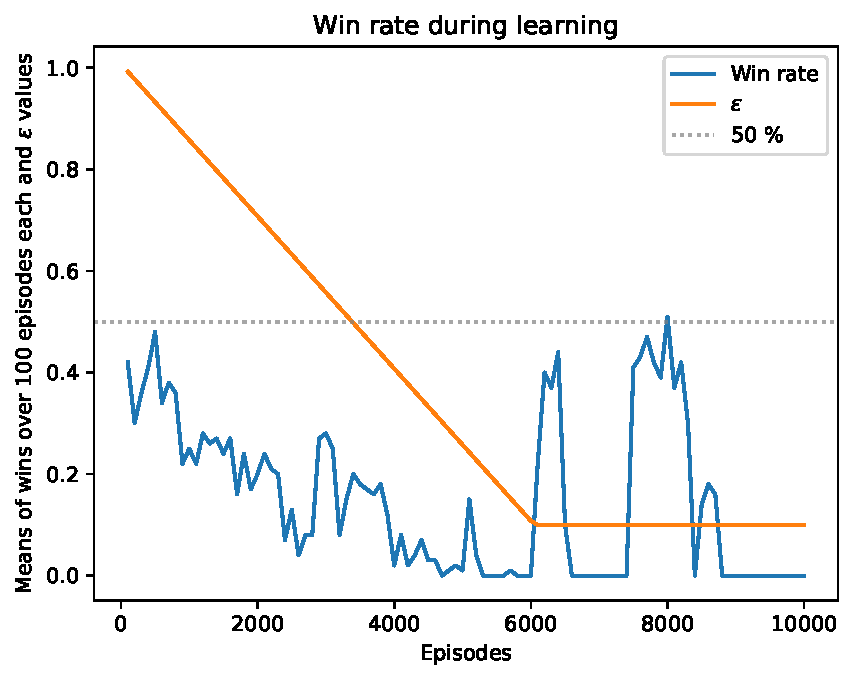
\includegraphics[width=\textwidth]{../experiments/exp3/win_stats.pdf}
  \caption{Results of experiment~3. Plotted in blue is the average win rate over 100~episodes each to show the change of win rate during training. The green line represents~$\epsilon$, the ratio of random actions taken during training. Dotted in grey is the 50~\%~win rate margin. I will forgo writing the detailed description of future graphs of this type because they will continually be used throughout this~section.}
  \label{fig:exp3}
\end{figure}

For this experiment and the future ones, the player count was reduced to two. Except for the learning rates which were reduced by a factor of~10 for both networks, setting them to~0.0001 and~0.001 for the actor and critic respectively, the parameters follow experiment~3. Removing the third player accelerated the simulations a lot: With about 0.76~seconds per episode, the experiment finished in a little over 2~hours. Achieving only very minor spikes in the win rate, Kraudia's results were absolutely unsatisfactory. Learning was not occurring and the wins can be attributed to~luck. \medskip

Therefore, change in the naive reward system was~necessary.

\subsection{Reward Sophistication and Breakthrough (5 to 9)}

For all following experiments, the reward system as explained in \hyperref[sec:rewards]{section~\ref*{sec:rewards}} was used. Because I was not ready to experiment yet, the feature type is still set to~2 for all experiments. Except when mentioned otherwise, experiments in this subsection use 50~neurons in the first hidden layer for both~networks.

Experiments~5 and~6 used a learning rate of~0.0001 for the actor and~0.001 for the critic. Also, both network's update factors were set to~0.001. The only difference in parameters is that experiment~6 uses 100~neurons in the first hidden layer for both networks.
Increasing the number of neurons proved to be important although with drawbacks: In contrast to experiment~5 in which results suddenly peaked at the end at about~50~\% after decreasing to zero before, experiment~6 shows much more stable learning. However, one of the aforementioned drawbacks is that at the end of experiment~6, the stability is no more and results start dropping. The other is that while experiment~5 finished in roughly 2~hours and 17~minutes with about 0.82~seconds per episode, experiment~6 took slightly over 7~hours with around 2.55~seconds per episode. This is a dramatic increase in run time easily explainable by the amount of parameters to train: With a feature vector of size~52 as in the experiments, two hidden layers with 50~neurons each result in 5\,350~parameters while having 100~neurons in the first and 50~neurons in the second layer results in 10\,450~trainable weights~--  almost twice as many. There is another reason for the huge increase in run time: Due to Kraudia playing better, games take a longer time to~finish.

Except for the changes mentioned at the beginning of this subsection, experiment~7 has the default parameters. Learning was less stable than in experiment~6 but when results peaked, they were almost constant (although sadly only for some thousand episodes). It took less than 4~hours for experiment~7 to complete with about 1.39~seconds per episode. Experiment~8 had the same parameters as experiment~7 except for the update factor which was reduced to~0.001 for both networks. This increased stability by a great deal. Results oscillated much less than in experiment~6 while achieving a win rate above~50~\% for some periods. Sadly, at the end results again suddenly dropped by a large~margin.

Combining the amount of neurons in experiment~6 and the learning rates and update factor in~7, we arrive at the default parameters (except for the feature type which is still~2) which were also used for experiment~9. I consider this experiment the breakthrough because not only did Kraudia achieve a stable win rate over~50~\% (after a few initial hiccups) but also the results did not drop at the end of the experiment suggesting that~-- hopefully~-- a more steady solution has been~found. Experiment~9 took over 8~hours to complete with almost 3~seconds per episode. Results are shown in \hyperref[fig:exp9]{figure~\ref*{fig:exp9}}.
\begin{figure}
  \centering
  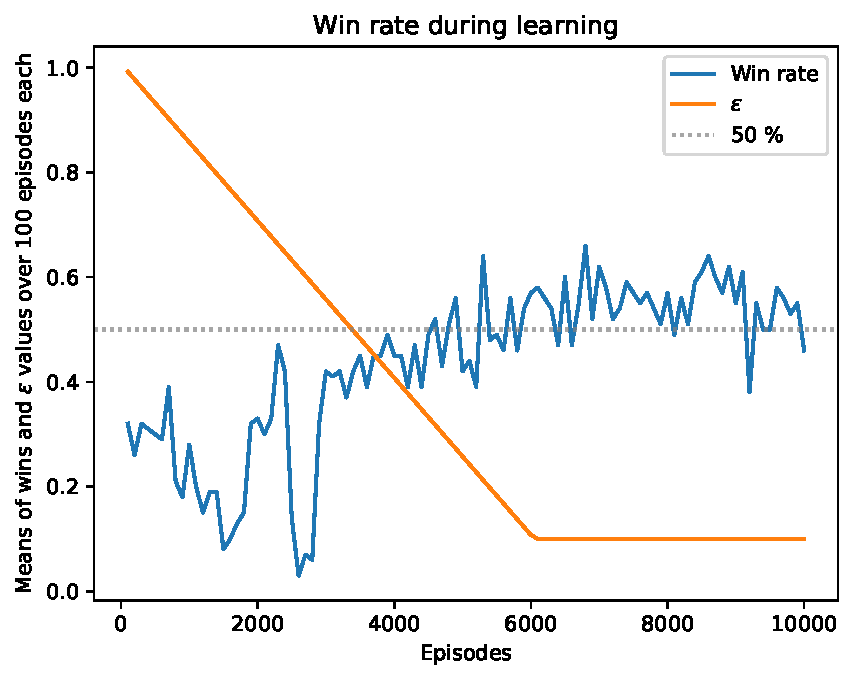
\includegraphics[width=\textwidth]{../experiments/exp9/win_stats.pdf}
  \caption{Results~of~experiment~9}
  \label{fig:exp9}
\end{figure}
\medskip

Looking at the past five experiments, a very interesting pattern can be found: The better the agent becomes, the longer the games take. The following numbers denote the amount of times the agent has learned from a batch from memory. Going from worst to best, in experiment~5 where bad results were observed (18.63~\%~total win rate), the network was trained about 79\,896~times. Experiment~7 had a total win rate that was roughly 9~percentage points~(pp) better and was trained 83\,938~times. For experiment~6, the amount of training increased to~90\,576 even though the total win rate was only almost 5~pp better. This is because the win rate~-- and subsequently game length~-- was much more stable during experiment~6. With a total win rate of~41.79~\% in experiment~8, the network was trained 92\,082~times. Experiment~9 takes the cake with 93\,993~training runs and a total win rate~of~43.29~\%.

\subsection{Further Parameter Tuning (10 to 20)}
\label{sec:tuning}

The default parameters are the starting point for the experiments of this subsection except for the feature type which is set to~2 up until~experiment~16.

To try and surpass the results of experiment~9, I increased the amount of neurons to~100 for the second layer as well, leading us to experiment~10. Results looked promising as learning was more stable than in experiment~9. Sadly, a sudden drop at episode~9\,000 nullified all previous learning as the agent was not able to return back to its high win rate during the last 1\,000~episodes, keeping the win rate close to~zero. Interestingly, experiment~10 completed over three hours faster than experiment~9 with only about 1.82~seconds per episode. It is not easy to say for certain what caused this. Maybe the network learned which actions were illegal more quickly or maybe simply fewer people were using the~computer.

The amount of neurons in both layers was swapped in experiment~11 (so we have 50~neurons in the first and~100 in the second layer for both networks) resulting in less stable learning. Ultimately, though, a win rate similar to experiment~9 was reached.

Next, I wanted to try weighting the amount of trump cards more. Sadly, experiment~12 is where I probably made a mistake documenting the parameters. I had $\epsilon$ start listed as 0.1. Looking at the win rate, this might not be true, though, as the win rate decreased with more episodes spiking only at the very end for a short time. On the other hand, the results were too bad for only changing a reward weight (to a value making sense, too) suggesting that something went wrong. My first impression was that the function was stuck at a local optimum so I redid the experiment. Ignoring what went wrong in the first try, the experiment ended after over 9~hours with approximately 3.32~seconds per episode. The results were similar to experiment 9. As there are only a few cards in the deck, changing the reward could not make a big difference. To speed up computation, I compiled TensorFlow from sources activating SSE4.1 and SSE4.2~(probably unnecessary) instructions which were available on all computers I could use for the calculations. The faster version was used from the second try of experiment~12 and~onward.

With experiment~13, I wanted to test an agent versus agent scenario but it took too long to complete and was subsequently cancelled.

Experiment~14 uses RMSProp as its optimizer with reward weights set to $w_v = 4$, $w_t = 3$, $w_c = 6$. Results continually decreased~-- either the parameters were not suited for RMSProp or RMSProp does not work well with DDPG. To test whether the reward weights might have influenced the result negatively, I recreated experiment~14 with Adam as the optimizer in experiment~15. After about 6~hours and 45~minutes with roughly 2.43~seconds per episode, it was clear that the reward weights were not fitting. The win rate oscillated heavily, reaching~0~\% during some periods and going above~50~\% during~others.

Finally, I decided to test feature type~1 bringing us to experiment~16  which uses the default parameters with no exceptions. With close to 3.11~seconds per episode, experiment~16 took over eight and a half hours. The time was well spent: Feature type~1 showed more stable results than feature type~2 and has the added benefit of resulting in a smaller feature vector which decreases computation time while the feature updates themselves are less computationally expensive as well. See \hyperref[fig:exp16]{figure~\ref*{fig:exp16}} for the results. It is also worth mentioning that experiment~16 uses the same parameters as experiment~9 except for the feature type. No better parameters were found in the experiments between.

Only after finishing all experiments did I notice that there was an error in feature type~2 that would cause the less stable results. While still being a relatively good feature vector, obviously this impacts all results using feature type~2. This might mean that feature type~1 does not cause better results than feature type~2, however, the benefit of decreased computation time is still a given, so using feature type~1 from now on is not a bad~choice.
\begin{figure}
  \centering
  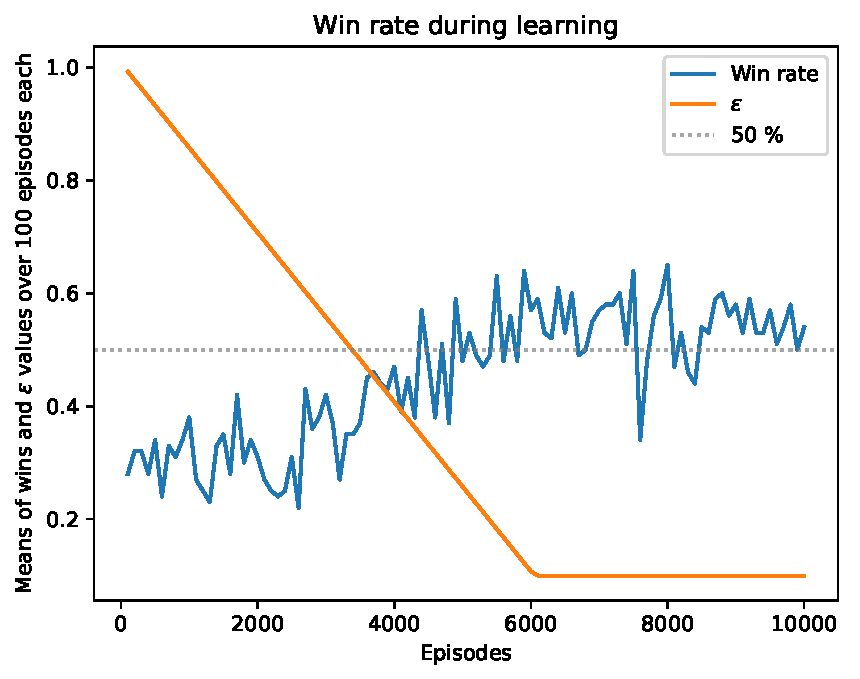
\includegraphics[width=\textwidth]{../experiments/exp16/win_stats.pdf}
  \caption{Results of experiment~16}
  \label{fig:exp16}
\end{figure}

Going forward from experiment~16, using feature type~1 for the rest of the experiments in this subsection, I wanted to optimize the $\varepsilon$ for numerical stability mentioned at the beginning of this section. Experiments~17,~18 and~19 have~$\varepsilon$ set to~$\expn{1}{-2}$,~$\expn{1}{-6}$ and~$\expn{1}{-10}$ respectively for both networks. Having the biggest deviance, experiment~17 achieves bad results while the other experiments, varying around the default of~$\expn{1}{-8}$, achieve similar results to experiment~16. We can also see that the long run time of experiment~16 had been caused by exterior factors: Both experiment~18 and~19 finished in a little over 4~hours and 50~minutes with around 1.76~seconds per~episode.

To try and fit the win and loss rewards more to the problem, taking in account that on average roughly 9.4~turns are played each game, I set the rewards for winning and losing to~8 and~$-8$ respectively for experiment~20. This negatively influenced the results instead of improving them. It lead to large oscillations suggesting that the agent needs a very influential reward at the end of a game so as to more correctly label its previous actions as good or~bad. \medskip

Even with all the parameter tuning in this section, I was not able to increase Kraudia's total win rate from experiment~9~(43.29~\%) by a lot (only experiments~16 with~44.99~\% and~18 with~43.87~\% rose above). Finally, realising that the problem was not that Kraudia did not learn enough but that the problem was most likely already solved, the game's parameters were modified to increase the complexity of the game. Because there are only twelve cards in the game and only three cards in hand, the game is bound to be more influenced by chance. I believe that Kraudia already played nearly optimally but could not reliably overcome the 60~\%~margin because even the random bots can win much based solely on luck in the downscaled version of durak that was used in all previous~experiments.

\subsection{Adding Complexity (21 to 33)}

From now on, I will mostly focus on full classic durak. The rules stay the same but the deck contains 36~cards and the players start with 6~cards in hand. To fit the parameters to the more complex and larger problem, the default parameters are now modified for all experiments in this subsection except when mentioned otherwise: We now let the agent learn for 5\,000~episodes instead of~10\,000 because games take much longer (the agent usually has more than twice as many training instances as before even though the episodes are halved). Correspondingly, $\epsilon$~episodes is also halved to be~3\,000 instead of~6\,000. The win and loss rewards are~36 and~$-36$ respectively to fit the deck~size.

For the very first experiment in this subsection, I let the agent learn full durak with 52~cards in the deck and 6~cards in hand. I used a win reward of 50 and a loss reward of $-50$. After almost exactly thirty and a half hours, taking around 21.96~seconds per episode, Kraudia achieved a total win rate of~56.20~\% and stuck at around 80~\%~win rate at the end. The results are found in \hyperref[fig:exp21]{figure~\ref*{fig:exp21}}. Since in the graph the oscillations in win rate are far less distinct, I assume that luck was in fact the reason for the unstable win rate during the prior experiments. I was very surprised by Kraudia's great success at adapting to the much harder, larger domain of the full game as so few tweaks have been made (only two parameters were changed). Learning was stable with only one drop at around 2\,000~episodes which was probably bad luck. During each game, on average 66.2~turns were played resulting in 330938~training~instances.
\begin{figure}
  \centering
  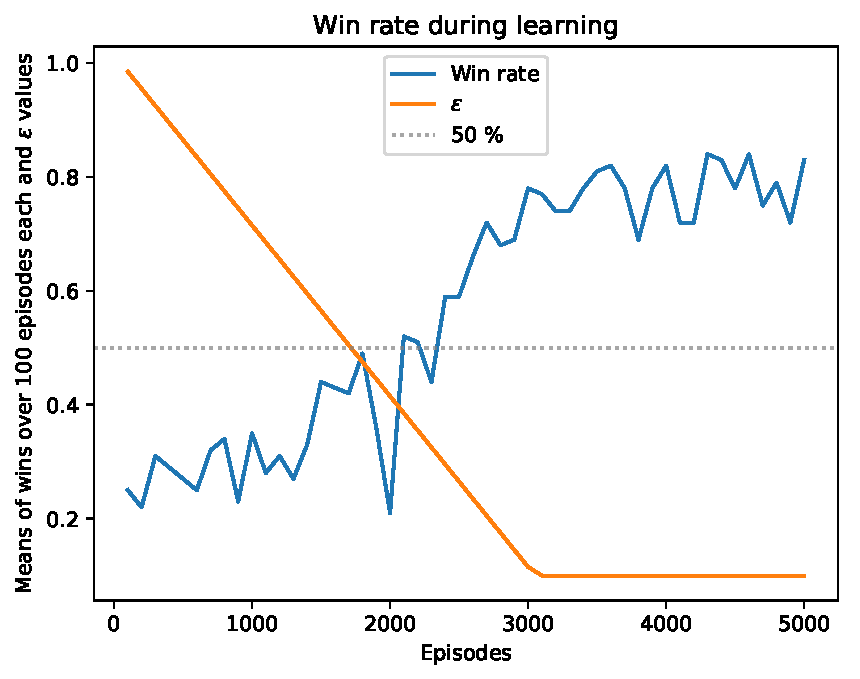
\includegraphics[width=\textwidth]{../experiments/exp21/win_stats.pdf}
  \caption{Results of experiment~21 for durak with 52~cards in deck}
  \label{fig:exp21}
\end{figure}

At the same time I started another experiment for full classic durak, also with win and loss rewards of~50 and~$-50$ respectively. Sadly, because of a mistake on my side, I cannot provide the time it took to complete and amount of training the networks had. The results, though, show that training was stable and successful: After episode~3\,000, Kraudia stays at a win rate of~about~70~\%.

From experiment~23 on I use the rewards mentioned at the beginning of this subsection. I also increased the number of neurons in the second hidden layer to~100 for both networks in hopes of finding more information in the larger feature vector. However, this had the opposite effect: Learning was destabilized and the win rate at the final episodes was also a little less than in the previous~experiment. The experiment finished in roughly 11~hours with 7.92~seconds per episode on~average.

In experiment~24 I continue the trend of more neurons by setting the amount of neurons to~120 in the first and~60 in the second layer for both networks. I also tried adjusting the reward weights by giving the amount of trumps more value ($w_c = 3$, previously~2). With approximately 8.32~seconds per episode, experiment~24 took more than eleven and a half hours to complete. The computation time necessary for the increased amount of weights seems to be wasted, though, as experiment~25 uses the same reward weights but the default amount of neurons and achieves nearly the same total win rate (actually even very slightly more). Experiment~25 took about 11~hours and 20~minutes with roughly 8.17~seconds per episode which is not that much faster considering there are much fewer neurons. Again, the run time can have been influenced by exterior factors so it is not safe to make assumptions based on~it.

Trying to reproduce the results of experiment~22 with the win and loss reward as the positive and negative deck size respectively, I started experiment~26. The total win rate was much higher (54.66~\%~versus~53.70~\%) so setting the win and loss rewards according to the deck size seems to be a good heuristic approach. The results, received after a little over 11~hours and 40~minutes (circa 8.41~seconds per episode), are shown in~\hyperref[fig:exp26]{figure~\ref*{fig:exp26}}.
\begin{figure}
  \centering
  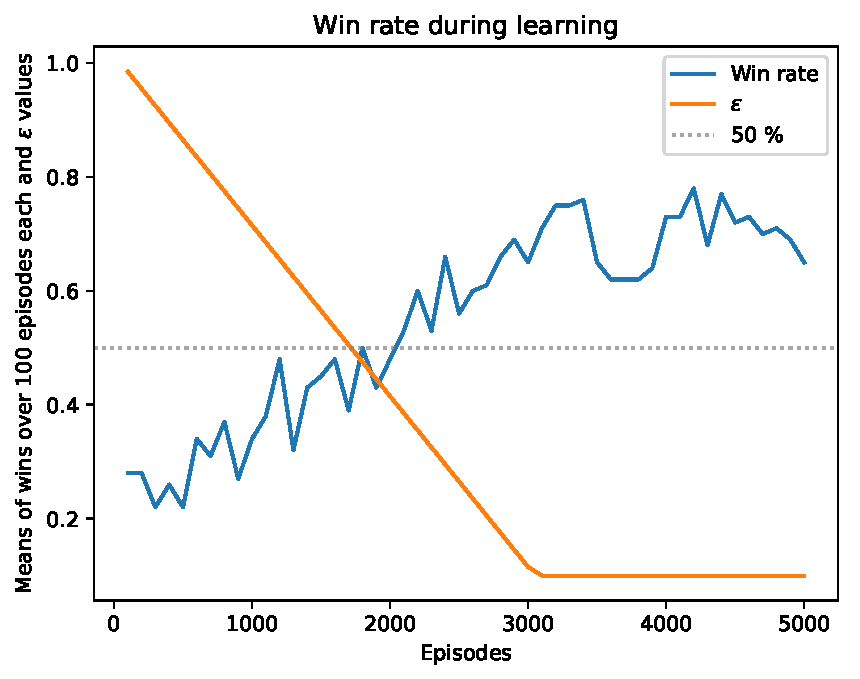
\includegraphics[width=\textwidth]{../experiments/exp26/win_stats.pdf}
  \caption{Results of experiment~26 for durak with 36~cards in deck}
  \label{fig:exp26}
\end{figure}

For the larger game versions, I have only used feature type~1 until now. Because it might prove to be worse than feature type~2, I now redo experiment~26 with the feature type set to~2. Taking only over 4~hours with around 2.98~seconds per episode, experiment~27 shows that feature type~2 does not only give worse results than feature type~1 but it might not be usable for the whole game at all. Whether it is not usable at all should be tested, though, as the win rate only falls off shortly after episode~2\,000 whereas prior to that it increases continuously with~decreasing~$\epsilon$.

Finally touching a parameter that has not been varied at all, in experiment~28 I set $\gamma$~to~0.5 instead of~0.99 which means that the agent does not look as far in the future. Surprisingly, after a little under 13~hours and 45~minutes with about 9.89~seconds per episode, the total win rate does not suffer meaningfully. This can have many interpretations. For example, it could be that the agent has not learned to plan at all which would correspond to the results in the Nature paper~\cite{nature} in which bad results were achieved for a game requiring planning and strategy. Another interpretation which can coexist with the first one is that maybe durak can be played well without planning much. However, this is hard to confirm as the rewards awarded during the game shape Kraudia's planning~behaviour.

As the reward weights can change a lot in Kraudia's behaviour and subsequently win rate, I try to give the amount of trumps much more value than the other weights by setting $w_t$~to~1 and $w_c$~to~3 in experiment~29. This negatively influences the total win rate compared to~experiment~26.

Sadly, experiment~30, which tested more than two players, was interrupted due to an error that was later fixed. Due to time constraints, I was not able to redo this experiment.

In experiments~31 and~32, I test whether more training increases Kraudia's win rate further by loading the network weights found by experiment~26. For experiment~31, I start with $\epsilon$~at~1 as usual to give the agent more random results to work with so it does not get stuck at its already found strategy. The total win rate is higher than in experiment~26 which is obvious considering that actions taken at the beginning are already much more refined. Experiment~31 took less than ten and a half hours with roughly 7.51~seconds per episode. In contrast, experiment~32, begins with $\epsilon$~at~0.1, meaning that training basically begins where it left off in experiment~26. Sadly, the results were terrible. Either loading only the weights (without the whole TensorFlow graph information) does not work well when keeping $\epsilon$ low at the beginning or Kraudia simply fails after too many experiments as the agent gets stuck with a bad~strategy. As with all experiments that end badly, experiment~32 took much less time to complete than a successful one. With not even 4~hours of run time and 2.76~seconds per episode on average, experiment~32 took less than half as long as its counterpart~experiment~31.

Up until now I have always used only two hidden layers to keep the computational effort low. However, I still wanted to improve the results so I add a third hidden layer with 25~neurons to both networks (neurons per layer is then [100, 50, 25] for both networks) in experiment~33. The run time exploded: With approximately 14.44~seconds per episode, the experiment took more than 20~hours to complete. Compared to experiment~26, the total win rate was better but not even by 1~pp which means that~-- for me~-- the extra layer and its additional computation time is not worth~it.

\newpage

\section{Conclusion}

The experiments show that Kraudia learns to play better than a player that simply acts at random. The win rate is not as high as expected for playing against a random bot. This could be because durak is based more on luck than expected or because the agent is simply not playing well enough. As this can be tested by letting the agent learn against itself, that is one of the next steps in refining the agent. Sadly, this also means that the question whether durak can be classified as a game of skill cannot yet be~answered.

Whether representing the cards' location by indices works for indices greater than one has to be tested with more players in the game. However, for two players it outclassed the binary card location representation not only by efficiency but by results as well. If the representation by indices applies to more than two players, a new, better representation for the location of cards in card games has been found and may be applied to other problems as well in which previously binary features had to be used. Since no more than two players were tested in depth, we also do not know how the agent would reply to multiple other players. Results could be completely different in the end. Also, it is interesting to test whether removing the minimal prior knowledge (see~\hyperref[sec:behaviour]{section~\ref*{sec:behaviour}}) greatly influences the result. This is especially important for more than two players as for only two players, it is always optimal to play with the implemented behaviour. Testing more than two players is also very important to verify and reinforce the results of this~thesis.

As mentioned in \hyperref[sec:tuning]{section~\ref*{sec:tuning}}, the results for feature type~2 are not completely correct and it should once again be tested against feature type~1 to find out whether it might actually be better.

All in all, most of the parameters were adequately fitted to the problem while the experiments remained relatively time efficient. It is obvious that a properly designed reward function had a big impact on the performance of the agent. After shaping the rewards, reinforcement learning actually~worked.

\subsection{Implementation Improvements}
\label{sec:improvements}

To make the agent play even more optimally, placing multiple cards at a time should be implemented. This could be done by implementing a new type of action that signals that another action follows. Actions and their cards could then be collected in a list and played all at once when the final action~-- signalling that no further action follows~-- is~chosen.

Obviously, a graphical user interface for human players should be added and it would be nice to be able to play against Kraudia online or even on a mobile phone. Using a graphical user interface, Kraudia could also predict which actions are how good by assigning different colors to each cards' actions. The code can be massively optimized to have the experiments end even~faster.

\subsection{Further Methods}

It would be interesting to try and apply \emph{hindsight experience replay}~\cite{her} to the game as hindsight experience replay does not require a shaped reward function (in the paper, it is actually advised against shaping the rewards). In fact, a reward function even more naive than the one that was tested at the very beginning of the experiment is all that is necessary~-- one that rewards $-1$ whenever the agent has not yet won and 1 when it has. Whether hindsight experience replay is actually applicable to the problem obviously remains to be tested but results would probably be better as fewer prior knowledge is required. However, as the agent might only try to win quickly (because of the negative reward at each time step), it might be less successful as~well.

For even more optimal play, we could apply subgame solving for imperfect-information games~\cite{subgame}, also used by the current best heads-up no-limit Texas hold'em poker~AI (called Libratus). This might not have as many uses for durak, though, as bluffing does not play as great a part in it and the game is more limited than poker in the sense that there is less variance in the players' actions (betting in poker is the best example for a lot of variance). However, to get the best and probably more stable results, subgame solving can also be taken into~account.

\subsection{Outlook}

Solving durak does not have practical scientific applications itself. However, understanding and applying reinforcement learning on a complex domain is knowledge useful for a lot of problems. Although on a domain that it was initially not invented for, the stability of the DDPG algorithm has once again been shown which is astounding considering that a continuous algorithm was applied to discrete parameters. In the future, even more complex, real time problems can be tackled using similar~techniques.

\newpage

\section{Appendix}
\label{sec:appendix}

The code is available online on GitHub at \url{github.com/janEbert/rldurak}. TensorFlow~\cite{tensorflow} and Keras~\cite{keras} have to be installed alongside Python~\cite{python} to execute the~program. \bigskip

\begin{table}[h]
\centering
  \begin{tabular}{lrl}
    \toprule
    Parameter & Value & Description \\
    \midrule
    episodes & 10\,000 \\
    feature type & 1 \\
    $\epsilon$~start & 1 & linearly anneal min~$\epsilon$ from this\\
    min~$\epsilon$ & 0.1 & $\epsilon$~does not decrease further than this \\
    $\epsilon$~episodes & 6\,000 & linearly anneal in this many episodes \\
    optimizer & Adam \\
    $\alpha$~actor & 0.001 & learning rate \\
    $\alpha$~critic & 0.01 \\
    $\varepsilon$~actor & $\expn{1}{-8}$ & $\varepsilon$~for numerical stability \\
    $\varepsilon$~critic & $\expn{1}{-8}$ \\
    $\tau$~actor & 0.01 & target model update factor \\
    $\tau$~critic & 0.01 \\
    neurons per layer~actor & [100, 50] & neurons in each hidden layer \\
    neurons per layer~critic & [100, 50] \\
    $\gamma$ & 0.99 & discount factor \\
    max experience count & 500 \\
    batch size & 32 \\
    win reward & 12 \\
    loss reward & $-12$ \\
    wait reward & $-0.05$ \\
    illegal action reward & $-100$ \\
    $w_v$ & 1 & weight for difference in mean card value \\
    $w_t$ & 2 & weight for difference in mean trump value \\
    $w_c$ & 2 & weight for difference in trump amount \\
    $\psi_\mu$ & 0.95 & mean value for how often bots wait \\
    $\psi_\sigma$ & 0.1 & standard deviation for how often bots wait \\
    $\chi_\mu$ & 0.08 & mean value for how often bots check \\
    $\chi_\sigma$ & 0.1 & standard deviation for bots checking \\
    wait until defended & true & agent attacking behaviour \\
    \bottomrule
  \end{tabular}
  \caption{Default parameters for the experiments}
  \label{table:parameters}
\end{table}

\newpage

\begin{thebibliography}{99}

\bibitem{mlquote}
  Ng, Andrew. ``Machine Learning.'' \emph{Coursera}. Machine Learning | Coursera, 2017. Web. 7~Nov.~2017.,
  \url{coursera.org/learn/machine-learning}

\bibitem{wikidurak}
  Wikipedia contributors. ``Durak.'' \emph{Wikipedia, The Free Encyclopedia}. Wikipedia, The Free Encyclopedia, 31~Aug.~2017. Web.
  7~Sep.~2017.,
  \url{en.wikipedia.org/w/index.php?title=Durak&oldid=798247605}

\bibitem{book}
  Sutton, Richard~S., and Andrew~G.\ Barto. ``Reinforcement Learning: An Introduction.'' \emph{Reinforcement Learning: An Introduction}. Rich Sutton's Home Page, 19~Jun.~2017. Web.
  20~Jun.~2017.,
  \url{incompleteideas.net/sutton/book/bookdraft2017june19.pdf}

\bibitem{nature}
  Mnih, Volodymyr, Koray Kavukcuoglu, David Silver, et al. ``Human-level control through deep reinforcement learning.'' \emph{Nature}. Nature, 518:~529-533, 26~Feb.~2015.

\bibitem{ddpg}
  Lillicrap, Timothy~P., Jonathan~J.\ Hunt, et al. ``Continuous control with deep reinforcement learning.'' \emph{arXiv.org}. arXiv:1509.02971v5, 29~Feb.~2016. Web.
  10~Sep.~2017.,
  \url{arxiv.org/abs/1509.02971v5}

\bibitem{python}
  van~Rossum, Guido, et al. ``Python.'' \emph{Python}. Python Software Foundation, 20~Feb.~1991. Web.
  2017.,
  \url{python.org}

\bibitem{keras}
  Chollet, Fran\c{c}ois, et al. ``Keras.'' \emph{Keras}. GitHub, 27~Mar.~2015. Web.
  2017.,
  \url{github.com/fchollet/keras}

\bibitem{tensorflow}
  Abadi, Martín, et al. ``TensorFlow: Large-scale machine learning on heterogenous systems.'' \emph{TensorFlow}. Google Brain Team, 9~Nov.~2015. Web.
  2017.,
  \url{tensorflow.org}

\bibitem{adam}
  Kingma, Diederik~P., and Jimmy~Lei Ba. ``Adam: A Method for Stochastic Optimization.'' \emph{arXiv.org}. arXiv:1412.6980v9, 30~Jan.~2017. Web.
  19~Sep.~2017.,
  \url{arxiv.org/abs/1412.6980v9}

\bibitem{rmsprop}
  Hinton, Geoffrey, Nitish Srivastava, Kevin Swersky. ``Neural Networks for Machine Learning.'' \emph{Department of Computer Science, University of Toronto}. CSC321 Winter~2014~-- Introduction to Neural Networks and Machine Learning, Lecture~6, 11~Feb.~2015, Web. 23~Sep.~2017.,
  \url{www.cs.toronto.edu/~tijmen/csc321/slides/lecture_slides_lec6.pdf}

\bibitem{torcs}
  Lau, Ben. ``Using Keras and Deep Deterministic Policy Gradient to play TORCS.'' \emph{GitHub Pages}. GitHub, 11~Oct.~2016. Web.
  8~Sep.~2017.,
  \url{yanpanlau.github.io/2016/10/11/Torcs-Keras.html}

\bibitem{tfadam}
  Google Brain Team. ``tf.train.AdamOptimizer.'' \emph{TensorFlow}. Google Brain Team, API~r1.3, 17~Aug.~2017. Web.
  23~Sep.~2017.,
  \url{tensorflow.org/api_docs/python/tf/train/AdamOptimizer}

\bibitem{her}
  Andrychowicz, Marcin, et al. ``Hindsight Experience Replay.'' \emph{arXiv.org}. arXiv:1707.01495v2, 10~Jul.~2017, Web.
  26~Sep.~2017.,
  \url{arxiv.org/abs/1707.01495v2}

\bibitem{subgame}
  Brown, Noam, Tuomas Sandholm. ``Safe and Nested Subgame Solving for Imperfect-Information Games.'' \emph{arXiv.org}. arXiv:1705.02955v2, 26~May~2017, Web. 2~Sep.~2017.,
  \url{arxiv.org/abs/1705.02955v2}

\end{thebibliography}

\end{document}